\section{Phân tích, tổng kết các phương pháp và hệ thống ví dụ}
\subsection{Ưu, nhược điểm của các phương pháp}
    
    \subsubsection{Ưu điểm chung}
        \begin{itemize}
            \item So với các phương pháp giải đúng, các phương pháp xấp xỉ có tính chất "self-correcting"\cite{nummethodMATLAB} - tự sửa lỗi, tức là sai số tính toán được sửa lại sau mỗi bước lặp.
            
            \item Trong một vài trường hợp, các phương pháp này hội tụ rất nhanh và có thời gian chạy nhanh hơn hẳn các phương pháp giải đúng.
        \end{itemize}

    \subsubsection{Phương pháp Newton}
        \par \textbf{Ưu điểm:}
        \begin{itemize}
            \item Tốc độ hội tụ rất nhanh khi xấp xỉ đầu thỏa mãn.
            \item Dễ cài đặt, thuật toán đơn giản, dẽ nhớ.
        \end{itemize}

        \par \textbf{Nhược điểm:} Rất khó tìm xấp xỉ đầu cho phương pháp này do yêu cầu của hệ số co q.

    \subsubsection{Phương pháp lặp Jacobi và lặp Gauss-Seidel}
        \par \textbf{Ưu điểm:}
        \begin{itemize}
            \item Có thể chọn xấp xỉ đầu bất kỳ
            \item Xấp xỉ đầu ảnh hưởng lớn đến hệ số co nên ta có thể điều chỉnh tốc độ hội tụ bằng xấp xỉ đầu.
        \end{itemize}
        
        \par \textbf{Nhược điểm:}
        \begin{itemize}
            \item Yêu cầu ma trận phải chéo trội.
            \item Thuật toán phức tạp, ít dùng trong thực tế khi lấy nghịch đảo ma trận.
        \end{itemize}

\subsection{Chọn xấp xỉ đầu cho các phương pháp}

    Trong báo cáo này, nhóm đề xuất 2 cách chọn xấp xỉ đầu cho các phương pháp nêu trên như sau:

    \begin{enumerate}[label=(\roman*)]
        \item \textbf{Sử dụng kết quả của các phương pháp giải đúng:} Do tính self-correcting của các phương pháp giải gần đúng, chúng ta có thể "chữa lại" kết quả của các phương pháp giải đúng như Gauss-Jordan, Cholesky,... bằng cách lấy kết quả của các phương pháp giải đúng làm đầu vào và xấp xỉ đầu cho các phương pháp giải gần đúng để cải thiện độ chính xác về tính toán cho các phương pháp giải đúng. Cách chọn xấp xỉ đầu này phù hợp với cả ba phương pháp Newton, Gauss-Seidel và Jacobi.
        
        \item \textbf{Một cách chọn xấp xỉ đầu cho phương pháp Newton:} Năm 1986, Victor Pan cùng với John H. Reif \cite{PanReif} đề xuất một phương pháp xấp xỉ đầu vào cho phương pháp Newton. Theo đó, ma trận xấp xỉ ban đầu sẽ được tính từ ma trận đề bài $A$ như sau:
        $$ X_{0} = \frac{A^{T}}{\left\lVert A \right\rVert_{1}\left\lVert A \right\rVert_{\infty}} $$
    \end{enumerate} 

    Trên cơ sở của mục (ii), nhóm đề xuất gói tìm xấp xỉ đầu của phương pháp Newton như sau:
    
    \IncMargin{1em}\begin{function}[H]
    \caption{getFirstApprox($A$)}
    \KwIn{Ma trận $A$}
    \KwOut{Ma trận $X_{0}$ thỏa mãn điều kiện hội tụ}
    \SetAlgoLined   
    \Begin{
        $ t1 \longleftarrow \left\lVert A \right\rVert_{1}  $ \;
        $ t2 \longleftarrow \left\lVert A \right\rVert_{\infty}  $ \;
        $ X_{0} \longleftarrow (\frac{A}{t1 * t2})^{T} $   \;
        
        \While{$ \left\lVert E - AX_{0} \right\rVert \geq 1 $}{
            $ X_{0} \longleftarrow X_{0}(2E - AX_{0}) $ \;
        }

        \KwRet{$X_{0}$}
    }         
\end{function}\DecMargin{1em}

    \newpage

\subsection{Hệ thống ví dụ}

    \textbf{Ví dụ 1:} Nghịch đảo ma trận sau:
    $$
        \begin{bmatrix}
            15 & 1  & 4  & -8 \\
            2  & 16 & 9  & 3  \\
            1  & -9 & 12 & 1  \\
            1  & 0  & 5  & 23 
        \end{bmatrix}
    $$
    Đây là ma trận chéo trội hàng, thỏa mãn điều kiện hội tụ của phương pháp Jacobi cũng như Gauss-Seidel. Khi chạy các thuật toán với ma trận này với sai số $10^{-15}$, ta được kết quả kèm ma trận tích của kết quả thu được với ma trận ban đầu như sau: 
    
    \begin{center}
        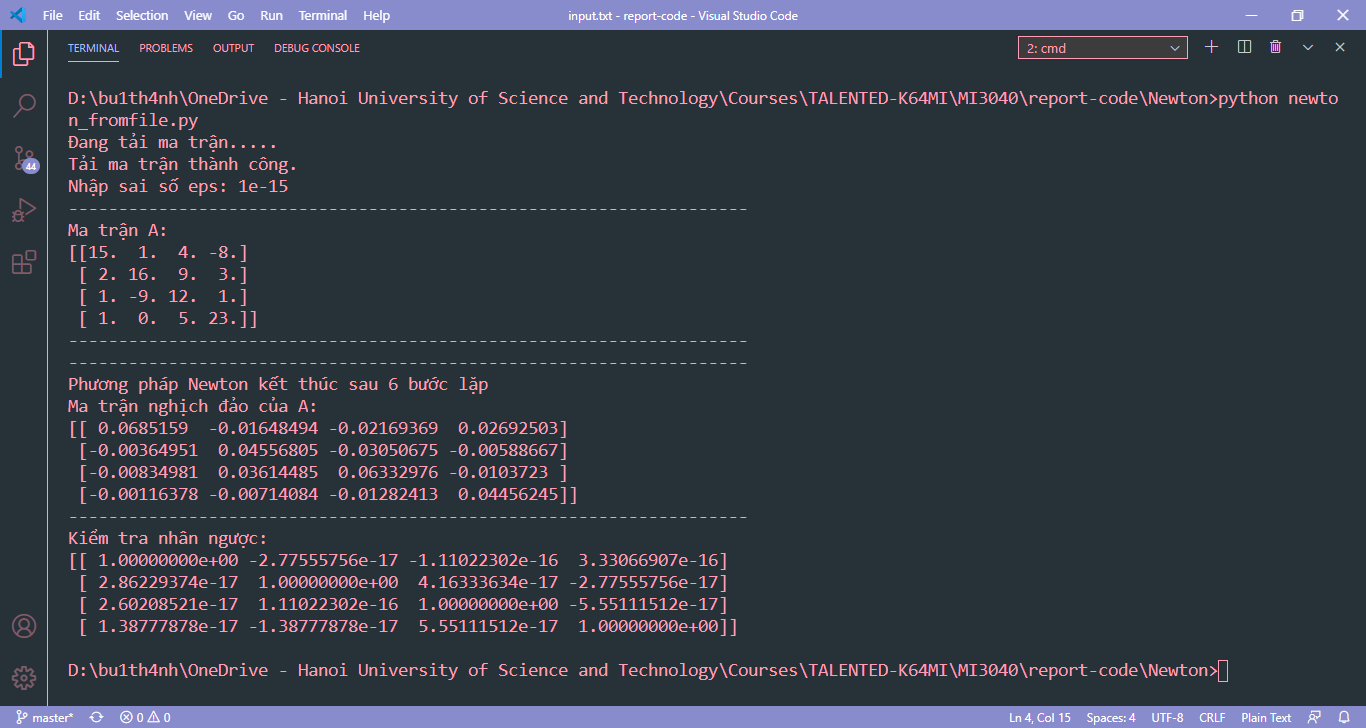
\includegraphics[scale=0.45]{example-02-newton.png} \\
        \textit{Phương pháp Newton với xấp xỉ đầu theo mục 5.2(ii)}
        
        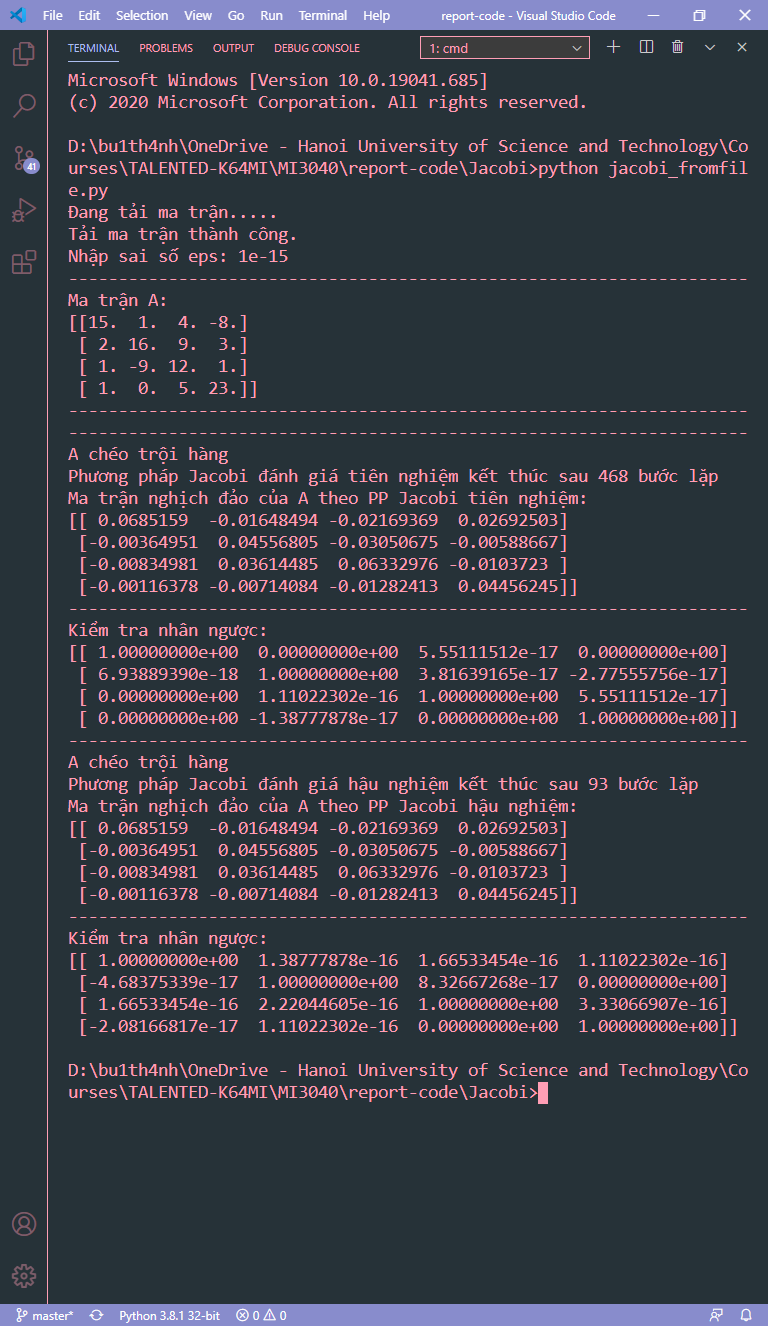
\includegraphics[scale=0.7]{example-02-jacobi.png} \\
        \textit{Phương pháp Jacobi, xấp xỉ đầu là ma trận A}
        
        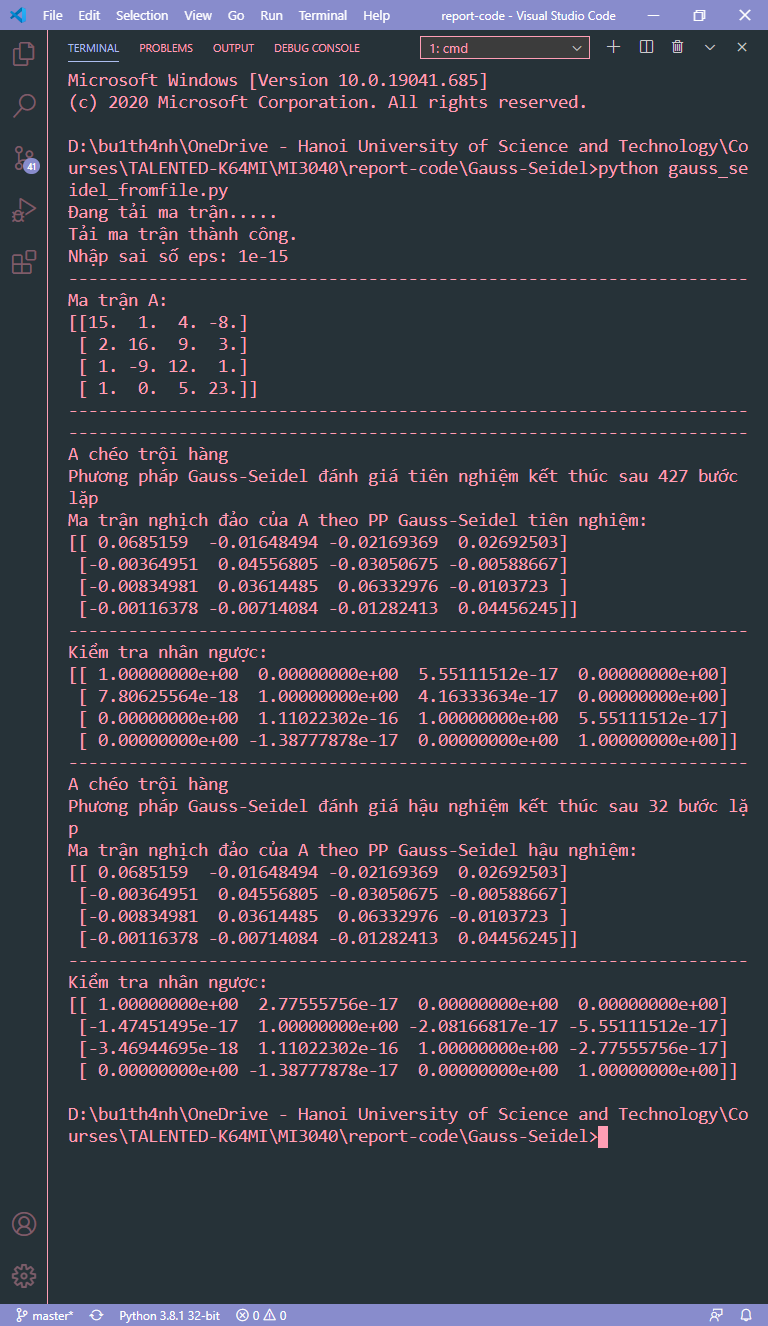
\includegraphics[scale=0.7]{example-02-gausseidel.png} \\
        \textit{Phương pháp Gauss-Seidel, xấp xỉ đầu là ma trận A}
    \end{center}

    Có thể thấy với xấp xỉ đầu là ma trận A, các phương pháp Jacobi và Gauss-Seidel có số bước lặp khá lớn do hệ số co phụ thuộc xấp xỉ đầu. Đây cũng là chủ đề nhóm sẽ cải tiến trong tương lai.
        


    \textbf{Ví dụ 2:} Nghịch đảo ma trận sau:
    $$
        \begin{bmatrix}
            0         & 5       & 0     & 0       \\
            0         & 0.00013 & 40    & 0       \\
            0         & 0       & 0.152 & 0.00067 \\
            0.00001 & 0       & 0     & 0
        \end{bmatrix}
    $$
    Đây là ma trận không chéo trội và có các định thức con chính bằng 0, tức là không thể chạy được với phương pháp viền quanh (chưa cải tiến) và các phương pháp Jacobi cũng như Gauss-Seidel. Khi chạy thuật toán Newton kèm cải tiến xấp xỉ đầu với ma trận này với sai số $10^{-15}$, ta được kết quả kèm ma trận tích của kết quả thu được với ma trận ban đầu như sau: 

    \begin{center}
        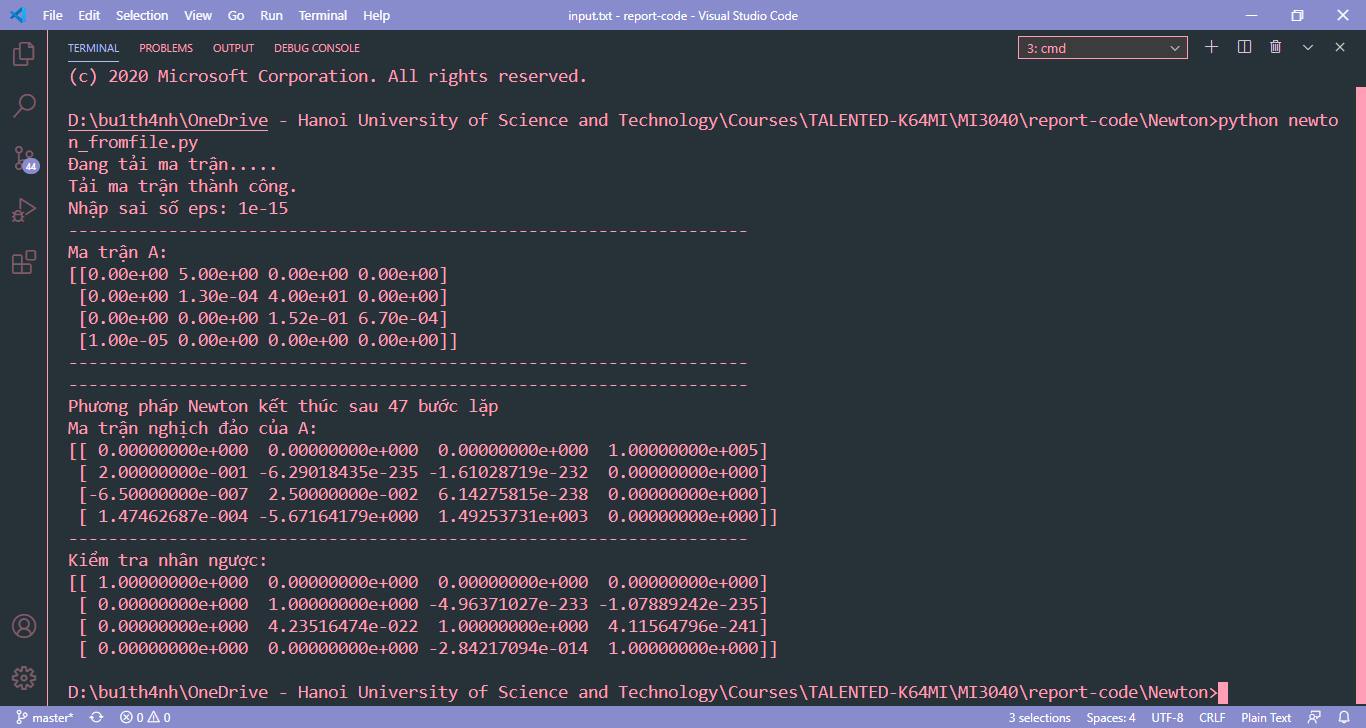
\includegraphics[scale=0.45]{example-01-newton.png}
    \end{center}


    \textbf{Ví dụ 3:} Nghịch đảo ma trận sau: \textit{(Ma trận gần suy biến)}
    $$
        \begin{bmatrix}
            3      & 2        & 7 \\
            2.0001 & 6.1      & 4 \\
            0      & 0.000001 & 0.001
        \end{bmatrix}
    $$
    Đây là ma trận chéo trội hàng và là ma trận gần suy biến, thỏa mãn điều kiện hội tụ của phương pháp Jacobi cũng như Gauss-Seidel. Khi chạy các thuật toán với ma trận này với sai số $10^{-15}$, ta được kết quả kèm ma trận tích của kết quả thu được với ma trận ban đầu như sau: 

    \begin{center}
        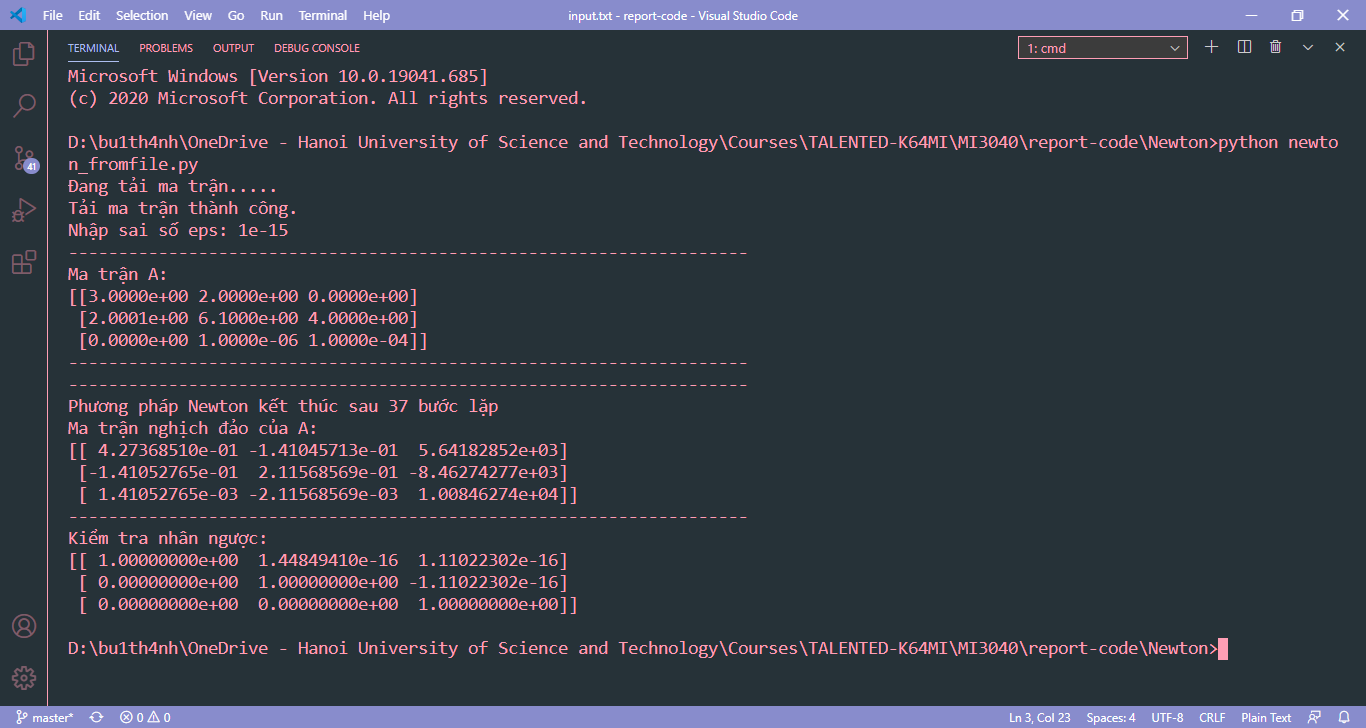
\includegraphics[scale=0.45]{example-03-newton.png} \\
        \textit{Phương pháp Newton với xấp xỉ đầu theo mục 5.2(ii)}
        
        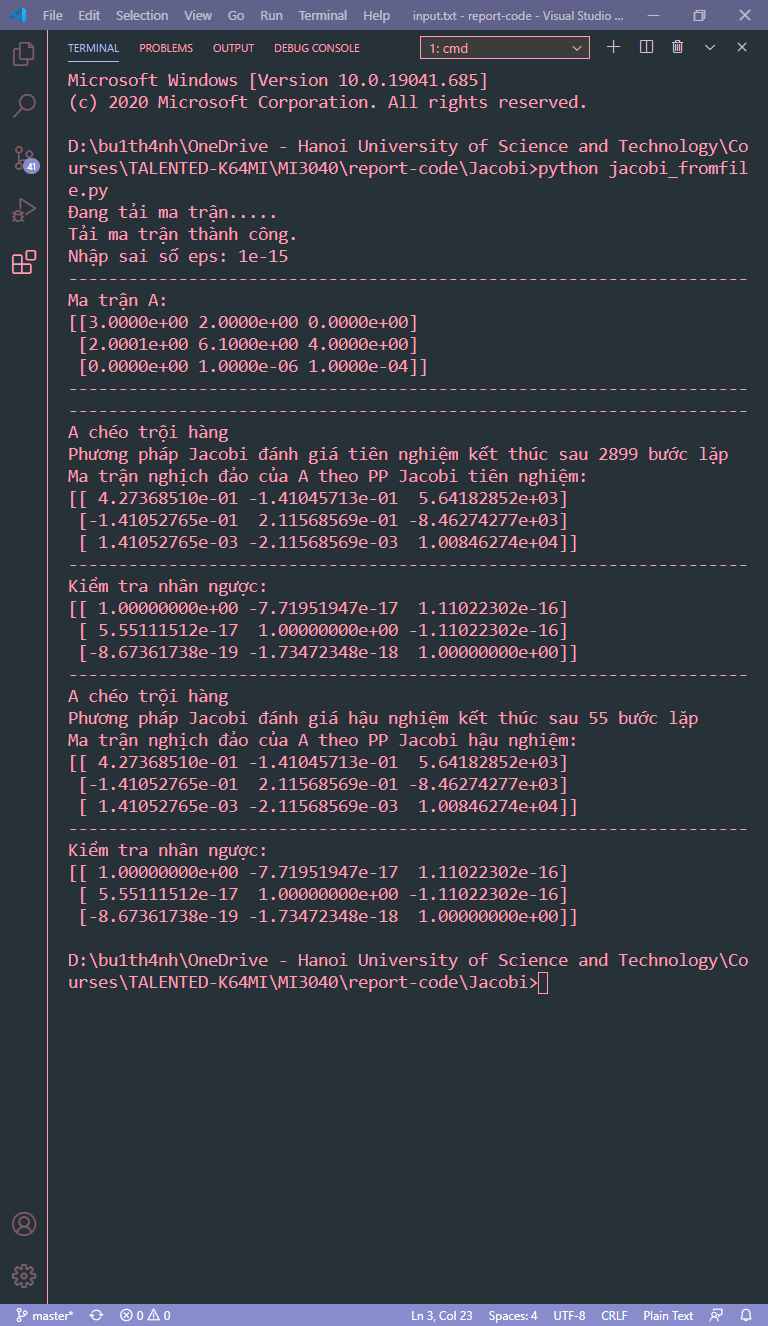
\includegraphics[scale=0.7]{example-03-jacobi.png} \\
        \textit{Phương pháp Jacobi, xấp xỉ đầu là ma trận A}
        
        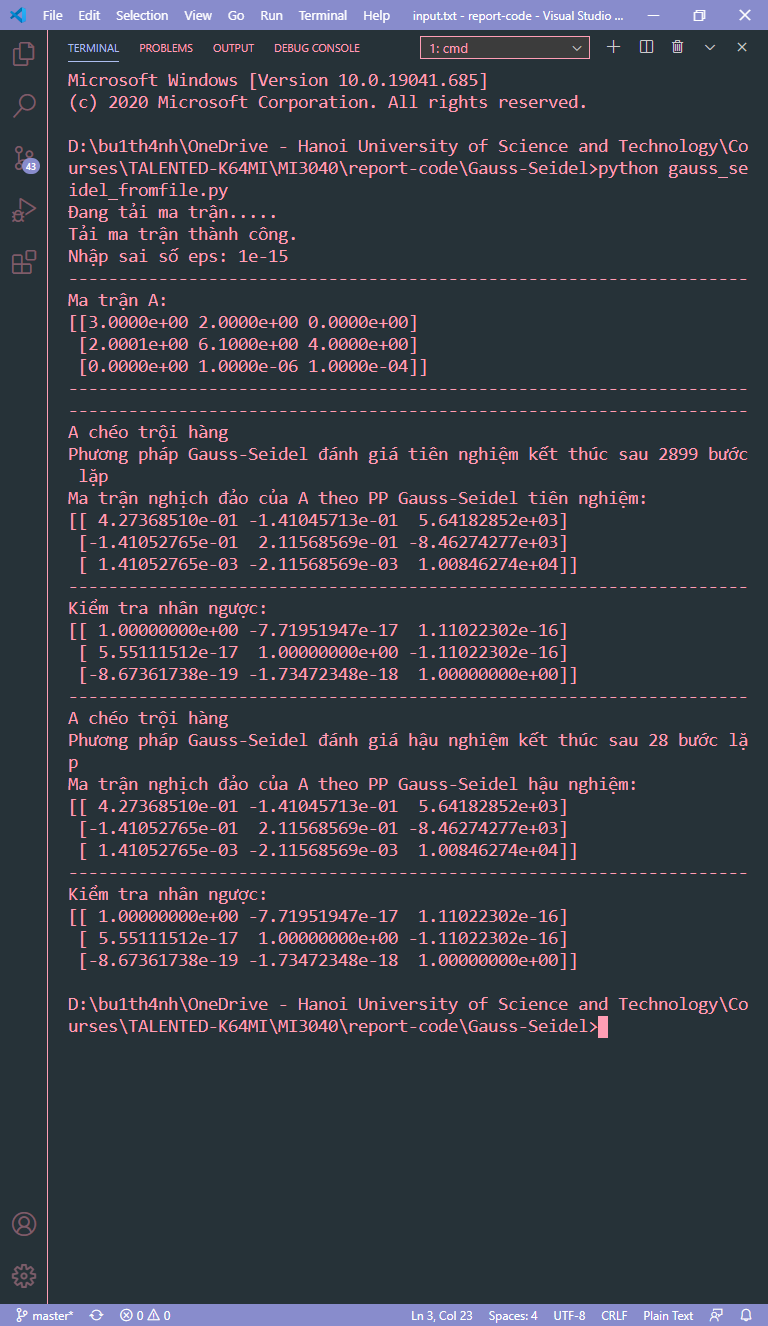
\includegraphics[scale=0.7]{example-03-gausseidel.png} \\
        \textit{Phương pháp Gauss-Seidel, xấp xỉ đầu là ma trận A}
    \end{center}

    Với hai phương pháp Jacobi và Gauss-Seidel, ví dụ này cho thấy sự khác biệt rõ rệt về số bước lặp giữa hai phương pháp tiên nghiệm và hậu nghiệm. Ở cả 2 phương pháp, cách đánh giá tiên nghiệm có số lần lặp gần 2900 bước, trong khi cách đánh giá hậu nghiệm có số lần lặp chưa đến 60 mà vẫn đảm bảo kết quả tương tự cách đánh giá tiên nghiệm. Ngoài ra, cả 3 phương pháp đều cho thấy sự ổn định khi ma trận có trạng thái gần suy biến.

\subsection{Ứng dụng}

    Nghịch đảo ma trận có rất nhiều ứng dụng trong thực tế. Chẳng hạn, có thể kể đến các ứng dụng như sau
    \begin{itemize}
        \item \textbf{Đồ họa máy tính:} Theo dõi một đối tượng trong không gian 3 chiều, có ứng dụng rất lớn trong ngành công nghiệp trò chơi điện tử, VFX và các ứng dụng VR,AR.
        \item \textbf{Kỹ thuật điện, điện tử:} Giải các hệ thống mạch điện
        \item \textbf{An toàn thông tin:} Mã hóa, giải mã thông tin
    \end{itemize}

    Đặc biệt, phương pháp Newton còn có thể sử dụng để tìm nghiệm của phương trình ma trận với ma trận hệ số không chéo trội - nhược điểm của các phương pháp lặp Jacobi, Gauss-Seidel để giải phương trình ma trận $AX = B$.
    
